\documentclass{article}
\usepackage{pgfplots}
\pgfplotsset{compat=newest}

\begin{document}

\begin{figure}[h]
    \centering
    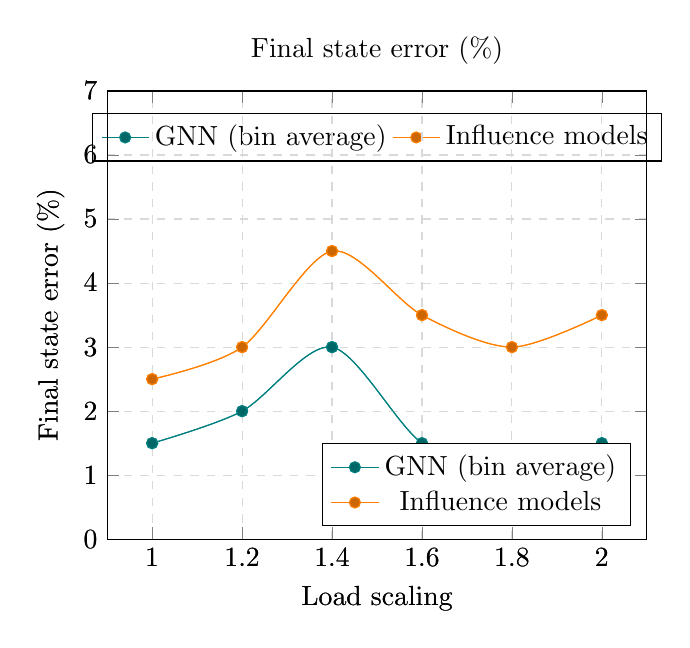
\begin{tikzpicture}
        \begin{axis}[
            title={Final state error (\%)},
            xlabel={Load scaling},
            ylabel={Final state error (\%)},
            legend style={at={(0.5,0.95)},anchor=north,legend columns=-1},
            ymin=0,
            ymax=7,
            xmin=0.9,
            xmax=2.1,
            xtick distance=0.2,
            ytick distance=1,
            grid=major,
            grid style={dashed, gray!30},
            ymajorgrids=true,
            enlargelimits=false,
            mark size=2pt,
            smooth,
            cycle list name=exotic,
            every node near coord/.append style={font=\tiny},
            point meta=explicit symbolic
        ]
            \addplot coordinates {
                (1.0, 1.5) [GNN (bin average)]
                (1.2, 2.0) [GNN (bin average)]
                (1.4, 3.0) [GNN (bin average)]
                (1.6, 1.5) [GNN (bin average)]
                (1.8, 1.0) [GNN (bin average)]
                (2.0, 1.5) [GNN (bin average)]
            };
            
            \addplot+[mark=*] coordinates {
                (1.0, 2.5) [Influence models]
                (1.2, 3.0) [Influence models]
                (1.4, 4.5) [Influence models]
                (1.6, 3.5) [Influence models]
                (1.8, 3.0) [Influence models]
                (2.0, 3.5) [Influence models]
            };
            \legend{GNN (bin average), Influence models}
        \end{axis}
        
        \begin{axis}[
            title={},
            xlabel={Load scaling},
            ylabel={Final state error (\%)},
            legend pos=south east,
            ymin=0,
            ymax=7,
            xmin=0.9,
            xmax=2.1,
            xtick distance=0.2,
            ytick distance=1,
            grid=major,
            grid style={dashed, gray!30},
            ymajorgrids=true,
            enlargelimits=false,
            mark size=2pt,
            smooth,
            cycle list name=exotic,
            every node near coord/.append style={font=\tiny},
            point meta=explicit symbolic
        ]
            \addplot coordinates {
                (1.0, 1.5) [GNN (bin average)]
                (1.2, 2.0) [GNN (bin average)]
                (1.4, 3.0) [GNN (bin average)]
                (1.6, 1.5) [GNN (bin average)]
                (1.8, 1.0) [GNN (bin average)]
                (2.0, 1.5) [GNN (bin average)]
            };
            
            \addplot+[mark=*] coordinates {
                (1.0, 2.5) [Influence models]
                (1.2, 3.0) [Influence models]
                (1.4, 4.5) [Influence models]
                (1.6, 3.5) [Influence models]
                (1.8, 3.0) [Influence models]
                (2.0, 3.5) [Influence models]
            };
            \legend{GNN (bin average), Influence models}
        \end{axis}
    \end{tikzpicture}
    \caption{Final state error rates $l_{state}^\alpha$ of various models for IEEE89 (left) and IEEE118 (right) against scaling values $\alpha$.}
    \label{fig:final_state_error}
\end{figure}

\end{document}